\documentclass{anstrans}
%%%%%%%%%%%%%%%%%%%%%%%%%%%%%%%%%%%
\title{Full-core multiphysics analysis of Molten Salt Reactor Experiment using parallel code}

\author{Andrei Rykhlevskii}

\email{andreir2@illinois.edu}

%%%% packages and definitions (optional)
\usepackage{graphicx} % allows inclusion of graphics
\usepackage{caption}  % allows center figures caption
\usepackage{booktabs} % nice rules (thick lines) for tables
\usepackage{microtype} % improves typography for PDF
\usepackage[section]{placeins}
\usepackage[acronym,toc]{glossaries}  % acronyms inclusion

%\newacronym{<++>}{<++>}{<++>}
\newacronym[longplural={metric tons of heavy metal}]{MTHM}{MTHM}{metric ton of heavy metal}
\newacronym{ABM}{ABM}{agent-based modeling}
\newacronym{ACDIS}{ACDIS}{Program in Arms Control \& Domestic and International Security}
\newacronym{AHTR}{AHTR}{Advanced High Temperature Reactor}
\newacronym{ANDRA}{ANDRA}{Agence Nationale pour la gestion des D\'echets RAdioactifs, the French National Agency for Radioactive Waste Management}
\newacronym{ANL}{ANL}{Argonne National Laboratory}
\newacronym{API}{API}{application programming interface}
\newacronym{ARCH}{ARCH}{autoregressive conditional heteroskedastic}
\newacronym{ARE}{ARE}{Aircraft Reactor Experiment}
\newacronym{ARFC}{ARFC}{Advanced Reactors and Fuel Cycles}
\newacronym{ARMA}{ARMA}{autoregressive moving average}
\newacronym{ASME}{ASME}{American Society of Mechanical Engineers}
\newacronym{ATWS}{ATWS}{Anticipated Transient Without Scram}
\newacronym{BDBE}{BDBE}{Beyond Design Basis Event}
\newacronym{BIDS}{BIDS}{Berkeley Institute for Data Science}
\newacronym{BOL}{BOL}{Beginning-of-Life}
\newacronym{BSD}{BSD}{Berkeley Software Distribution}
\newacronym{CAFCA}{CAFCA}{Code for Advanced Fuel Cycles Assessment}
\newacronym{CASL}{CASL}{Consortium for Advanced Simulation of Light Water Reactors}
\newacronym{CDTN}{CDTN}{Centro de Desenvolvimento da Tecnologia Nuclear}
\newacronym{CEA}{CEA}{Commissariat \`a l'\'Energie Atomique et aux \'Energies Alternatives}
\newacronym{CFD}{CFD}{Computational Fluid Dynamics}
\newacronym{CG}{CG}{Continuous Galerkin}
\newacronym{CI}{CI}{continuous integration}
\newacronym{CNEN}{CNEN}{Comiss\~{a}o Nacional de Energia Nuclear}
\newacronym{CNERG}{CNERG}{Computational Nuclear Engineering Research Group}
\newacronym{COMSOL}{COMSOL}{COMmon SOLution}
\newacronym{COSI}{COSI}{Commelini-Sicard}
\newacronym{COTS}{COTS}{commercial, off-the-shelf}
\newacronym{CSNF}{CSNF}{commercial spent nuclear fuel}
\newacronym{CTAH}{CTAHs}{Coiled Tube Air Heaters}
\newacronym{CUBIT}{CUBIT}{CUBIT Geometry and Mesh Generation Toolkit}
\newacronym{CURIE}{CURIE}{Centralized Used Fuel Resource for Information Exchange}
\newacronym{DAG}{DAG}{directed acyclic graph}
\newacronym{DANESS}{DANESS}{Dynamic Analysis of Nuclear Energy System Strategies}
\newacronym{DBE}{DBE}{Design Basis Event}
\newacronym{DESAE}{DESAE}{Dynamic Analysis of Nuclear Energy Systems Strategies}
\newacronym{DG}{DG}{Discontinuous Galerkin}
\newacronym{DHS}{DHS}{Department of Homeland Security}
\newacronym{DOE}{DOE}{Department of Energy}
\newacronym{DRACS}{DRACS}{Direct Reactor Auxiliary Cooling System}
\newacronym{DRE}{DRE}{dynamic resource exchange}
\newacronym{DSNF}{DSNF}{DOE spent nuclear fuel}
\newacronym{DYMOND}{DYMOND}{Dynamic Model of Nuclear Development }
\newacronym{EBS}{EBS}{Engineered Barrier System}
\newacronym{EDZ}{EDZ}{Excavation Disturbed Zone}
\newacronym{EIA}{EIA}{U.S. Energy Information Administration}
\newacronym{EPA}{EPA}{Environmental Protection Agency}
\newacronym{EP}{EP}{Engineering Physics}
\newacronym{FCO}{FCO}{Fuel Cycle Options}
\newacronym{FCT}{FCT}{Fuel Cycle Technology}
\newacronym{FEHM}{FEHM}{Finite Element Heat and Mass Transfer}
\newacronym{FEPs}{FEPs}{Features, Events, and Processes}
\newacronym{FHR}{FHR}{Fluoride-Salt-Cooled High-Temperature Reactor}
\newacronym{FLiBe}{FLiBe}{Fluoride-Lithium-Beryllium}
\newacronym{GCAM}{GCAM}{Global Change Assessment Model}
\newacronym{GDSE}{GDSE}{Generic Disposal System Environment}
\newacronym{GDSM}{GDSM}{Generic Disposal System Model}
\newacronym{GENIUSv1}{GENIUSv1}{Global Evaluation of Nuclear Infrastructure Utilization Scenarios, Version 1}
\newacronym{GENIUSv2}{GENIUSv2}{Global Evaluation of Nuclear Infrastructure Utilization Scenarios, Version 2}
\newacronym{GENIUS}{GENIUS}{Global Evaluation of Nuclear Infrastructure Utilization Scenarios}
\newacronym{GPAM}{GPAM}{Generic Performance Assessment Model}
\newacronym{GRSAC}{GRSAC}{Graphite Reactor Severe Accident Code}
\newacronym{GUI}{GUI}{graphical user interface}
\newacronym{HLW}{HLW}{high level waste}
\newacronym{HPC}{HPC}{high-performance computing}
\newacronym{HTC}{HTC}{high-throughput computing}
\newacronym{HTGR}{HTGR}{High Temperature Gas-Cooled Reactor}
\newacronym{IAEA}{IAEA}{International Atomic Energy Agency}
\newacronym{IEMA}{IEMA}{Illinois Emergency Mangament Agency}
\newacronym{INL}{INL}{Idaho National Laboratory}
\newacronym{IPRR1}{IRP-R1}{Instituto de Pesquisas Radioativas Reator 1}
\newacronym{IRP}{IRP}{Integrated Research Project}
\newacronym{ISFSI}{ISFSI}{Independent Spent Fuel Storage Installation}
\newacronym{ISRG}{ISRG}{Independent Student Research Group}
\newacronym{JFNK}{JFNK}{Jacobian-Free Newton Krylov}
\newacronym{LANL}{LANL}{Los Alamos National Laboratory}
\newacronym{LBNL}{LBNL}{Lawrence Berkeley National Laboratory}
\newacronym{LCOE}{LCOE}{levelized cost of electricity}
\newacronym{LDRD}{LDRD}{laboratory directed research and development}
\newacronym{LFR}{LFR}{Lead-Cooled Fast Reactor}
\newacronym{LGPL}{LGPL}{Lesser GNU Public License}
\newacronym{LLNL}{LLNL}{Lawrence Livermore National Laboratory}
\newacronym{LMFBR}{LMFBR}{Liquid-Metal-cooled Fast Breeder Reactor}
\newacronym{LOFC}{LOFC}{Loss of Forced Cooling}
\newacronym{LOHS}{LOHS}{Loss of Heat Sink}
\newacronym{LOLA}{LOLA}{Loss of Large Area}
\newacronym{LP}{LP}{linear program}
\newacronym{LWR}{LWR}{Light Water Reactor}
\newacronym{MARKAL}{MARKAL}{MARKet and ALlocation}
\newacronym{MA}{MA}{minor actinide}
\newacronym{MCNP}{MCNP}{Monte Carlo N-Particle code}
\newacronym{MILP}{MILP}{mixed-integer linear program}
\newacronym{MIT}{MIT}{the Massachusetts Institute of Technology}
\newacronym{MOAB}{MOAB}{Mesh-Oriented datABase}
\newacronym{MOOSE}{MOOSE}{Multiphysics Object-Oriented Simulation Environment}
\newacronym{MOX}{MOX}{mixed oxide}
\newacronym{MPI}{MPI}{Message Passing Interface}
\newacronym{MSBR}{MSBR}{Molten Salt Breeder Reactor}
\newacronym{MSFR}{MSFR}{Molten Salt Fast Reactor}
\newacronym{MSRE}{MSRE}{Molten Salt Reactor Experiment}
\newacronym{MSR}{MSR}{Molten Salt Reactor}
\newacronym{NAGRA}{NAGRA}{National Cooperative for the Disposal of Radioactive Waste}
\newacronym{NCSA}{NCSA}{National Center for Supercomputing Applications}
\newacronym{NEAMS}{NEAMS}{Nuclear Engineering Advanced Modeling and Simulation}
\newacronym{NEUP}{NEUP}{Nuclear Energy University Programs}
\newacronym{NFCSim}{NFCSim}{Nuclear Fuel Cycle Simulator}
\newacronym{NFC}{NFC}{Nuclear Fuel Cycle}
\newacronym{NGNP}{NGNP}{Next Generation Nuclear Plant}
\newacronym{NMWPC}{NMWPC}{Nuclear MW Per Capita}
\newacronym{NNSA}{NNSA}{National Nuclear Security Administration}
\newacronym{NPRE}{NPRE}{Department of Nuclear, Plasma, and Radiological Engineering}
\newacronym{NQA1}{NQA-1}{Nuclear Quality Assurance - 1}
\newacronym{NRC}{NRC}{Nuclear Regulatory Commission}
\newacronym{NSF}{NSF}{National Science Foundation}
\newacronym{NSSC}{NSSC}{Nuclear Science and Security Consortium}
\newacronym{NUWASTE}{NUWASTE}{Nuclear Waste Assessment System for Technical Evaluation}
\newacronym{NWF}{NWF}{Nuclear Waste Fund}
\newacronym{NWTRB}{NWTRB}{Nuclear Waste Technical Review Board}
\newacronym{OCRWM}{OCRWM}{Office of Civilian Radioactive Waste Management}
\newacronym{ORION}{ORION}{ORION}
\newacronym{ORNL}{ORNL}{Oak Ridge National Laboratory}
\newacronym{PARCS}{PARCS}{Purdue Advanced Reactor Core Simulator}
\newacronym{PBAHTR}{PB-AHTR}{Pebble Bed Advanced High Temperature Reactor}
\newacronym{PBFHR}{PB-FHR}{Pebble-Bed Fluoride-Salt-Cooled High-Temperature Reactor}
\newacronym{PEI}{PEI}{Peak Environmental Impact}
\newacronym{PH}{PRONGHORN}{PRONGHORN}
\newacronym{PRKE}{PRKE}{Point Reactor Kinetics Equations}
\newacronym{PSPG}{PSPG}{Pressure-Stabilizing/Petrov-Galerkin}
\newacronym{PWAR}{PWAR}{Pratt and Whitney Aircraft Reactor}
\newacronym{PWR}{PWR}{Pressurized Water Reactor}
\newacronym{PetSc}{PetSc}{Portable, Extensible Toolkit for Scientific Computation}
\newacronym{PyNE}{PyNE}{Python toolkit for Nuclear Engineering}
\newacronym{PyRK}{PyRK}{Python for Reactor Kinetics}
\newacronym{QA}{QA}{quality assurance}
\newacronym{RDD}{RD\&D}{Research Development and Demonstration}
\newacronym{RD}{R\&D}{Research and Development}
\newacronym{RELAP}{RELAP}{Reactor Excursion and Leak Analysis Program}
\newacronym{RIA}{RIA}{Reactivity Insertion Accident}
\newacronym{RIF}{RIF}{Region-Institution-Facility}
\newacronym{SFR}{SFR}{Sodium-Cooled Fast Reactor}
\newacronym{SINDAG}{SINDA{\textbackslash}G}{Systems Improved Numerical Differencing Analyzer $\backslash$ Gaski}
\newacronym{SKB}{SKB}{Svensk K\"{a}rnbr\"{a}nslehantering AB}
\newacronym{SNF}{SNF}{spent nuclear fuel}
\newacronym{SNL}{SNL}{Sandia National Laboratory}
\newacronym{STC}{STC}{specific temperature change}
\newacronym{SUPG}{SUPG}{Streamline-Upwind/Petrov-Galerkin}
\newacronym{SWF}{SWF}{Separations and Waste Forms}
\newacronym{SWU}{SWU}{Separative Work Unit}
\newacronym{TRIGA}{TRIGA}{Training Research Isotope General Atomic}
\newacronym{TRISO}{TRISO}{Tristructural Isotropic}
\newacronym{TSM}{TSM}{Total System Model}
\newacronym{TSPA}{TSPA}{Total System Performance Assessment for the Yucca Mountain License Application}
\newacronym{ThOX}{ThOX}{thorium oxide}
\newacronym{UFD}{UFD}{Used Fuel Disposition}
\newacronym{UML}{UML}{Unified Modeling Language}
\newacronym{UOX}{UOX}{uranium oxide}
\newacronym{UQ}{UQ}{uncertainty quantification}
\newacronym{US}{US}{United States}
\newacronym{UW}{UW}{University of Wisconsin}
\newacronym{VISION}{VISION}{the Verifiable Fuel Cycle Simulation Model}
\newacronym{VV}{V\&V}{verification and validation}
\newacronym{WIPP}{WIPP}{Waste Isolation Pilot Plant}
\newacronym{YMR}{YMR}{Yucca Mountain Repository Site}
\newacronym{gpm}{gpm}{gallons per minute}

\graphicspath{{figures/}}
\captionsetup{justification   = raggedright,
              singlelinecheck = false}
\newcommand{\SN}{S$_N$}
\renewcommand{\vec}[1]{\bm{#1}} %vector is bold italic
\newcommand{\vd}{\bm{\cdot}} % slightly bold vector dot
\newcommand{\grad}{\vec{\nabla}} % gradient
\newcommand{\ud}{\mathop{}\!\mathrm{d}} % upright derivative symbol
\makeglossaries

\begin{document}
%%%%%%%%%%%%%%%%%%%%%%%%%%%%%%%%%%%%%%%%%%%%%%%%%%%%%%%%%%%%%%%%%%%%%%%%%%%%%%%%
\section{Introduction}
The \gls{MSR} is an advanced type of reactor which was developed at \gls{ORNL} 
in the 1950s and was operated in the 1960s. In the MSR, fluorides of fissile 
and/or fertile materials (i.e. UF$_4$, PuF$_3$ and/or ThF$_4$) are mixed with 
carrier salts to form a liquid fuel which is circulated in a loop-type primary 
circuit \cite{haubenreich_experience_1970}. This innovation leads to immediate 
advantages over traditional, solid-fueled, reactors. These include 
near-atmospheric pressure in the primary loop, relatively high coolant 
temperature, outstanding neutron economy, a high level of inherent safety, 
reduced fuel preprocessing, and the ability to continuously remove fission 
products and add fissile and/or fertile elements \cite{leblanc_molten_2010}. 

%%%%%%%%%%%%%%%%%%%%%%%%%%%%%%%%%%%%%%%%%%%%%%%%%%%%%%%%%%%%%%%%%%%%%%%%%%%%%%%%
\section{LITERATURE REVIEW}
\gls{MSR} modeling efforts describe steady-state and
transient behavior. Krepel et al. extended the in-house \gls{LWR}
diffusion code DYN3D to consider drift of delayed neutron precursors alongside
the reactor temperature profile, re-casting the extended code as
DYN3D-MSR \cite{krepel_dyn3d-msr_2007}. That work compared DYN3D-MSR against
experimental \gls{MSRE} data and then used it to simulate local fuel channel
blockages as well as local temperature perturbations. In a similar vein, Kophazi
et. al. used iterative coupling between in-house three-dimensional neutronic and
one-dimensional heat conduction models DALTON and THERM to analyze normal 
\gls{MSRE} operation as well as channel-blocking-incident
transients \cite{kophazi_development_2009}. The Kophazi model added entrance 
effects of heat transfer coefficients as well as thermal
coupling between fuel channels through moderator heat conduction. More recently,
Cammi et. al. performed a 2D-axisymmetric single-channel analysis of the
\gls{MSBR} using the commercial finite element package COMSOL
Multiphysics \cite{cammi_multi-physics_2011}. That work directly solved the 
fuel salt velocity field, used heterogeneous group constants
in fuel and moderator regions, and employed a software package (COMSOL)
intrinsically designed for coupled multi-physics simulation.
Additionally, Aufiero et. al \cite{aufiero_development_2014} have begun to 
approach transient simulations in the \gls{MSFR} by directly coupling Serpent 2 
Monte Carlo neutronics with OpenFOAM \cite{weller_tensorial_1998} thermal-hydraulics.

\section{Approach and method}
Recently developed multiphysics code Moltres
\cite{lindsay_moltres_2017} could be employed for simulating \glspl{MSR}.  By implementing
deterministic neutronics and thermal hydraulics in the context of the
\gls{MOOSE} finite element modeling framework, Moltres solves arbitrary-group
neutron diffusion, temperature, and precursor governing equations in anywhere
from one to three dimensions and can be deployed on an arbitrary number of
processing units. Through its computing power, Moltres is devoted to previously
unmatched fidelity in coupled neutronics and thermal hydraulics \gls{MSR}
simulation.

Moreover, Moltres depends on the \gls{MOOSE} framework, \cite{gaston_physics-based_2015} which is \gls{LGPL} code that itself 
leans on LibMesh \cite{kirk_libmesh:_2006}, a \gls{LGPL} finite element library, and PetSc \cite{satish_balay_petsc_2015}, a
\gls{BSD}-licensed toolkit for solving nonlinear equations yielded by 
discretizing PDEs. \gls{MOOSE} and LibMesh translate weak PDE forms defined by applications (e.g. Moltres) into residual and Jacobian functions. These functions are the inputs into PetSc Newton-Raphson solution routines. All codes use MPI for parallel communication and are easily deployed on massively-parallel cluster-computing platforms. \gls{MOOSE} applications by
default use monolithic and implicit methods ideal for closely-coupled and multi-scale physics, such as the model problem described in this work. However, Moltres can also use explicit time-stepping routines as well as segregated solution methods, making it extensible to myriad future modeling challenges.

In Moltres, neutrons are described with time-dependent multi-group diffusion theory: 

\hspace*{-0.7cm} 
$\frac{1}{v_g}\frac{\partial \phi_g}{\partial t} - \nabla \cdot D_g
\nabla \phi_g + \Sigma_g^r \phi_g = 
\chi_g^p \sum_{g' = 1}^G (1 - \beta) \nu \Sigma_{g'}^f \phi_{g'} + $
\begin{equation}
\sum_{g \ne g'}^G \Sigma_{g'\rightarrow g}^s \phi_{g'}
+ \chi_g^d \sum_i^I \lambda_i C_i
\end{equation}

\hspace*{-0.7cm} 
$v_g = \mbox{speed of neutrons in group g} \\
        \phi_g = \mbox{flux of neutrons in group g} \\
        t = \mbox{time} \\
        D_g = \mbox{diffusion coefficient for neutrons in group g} \\
        \Sigma_g^r = \mbox{macro removal cross-section from group g} \\
        \Sigma_{g'\rightarrow g}^s = \mbox{macroscopic cross-section of
        scattering from g' to g} \\
        \chi_g^p = \mbox{prompt fission spectrum, neutrons in group g} \\
        G = \mbox{number of discrete groups, g} \\
        \nu = \mbox{number of neutrons produced per fission} \\
        \Sigma_g^f = \mbox{macro cross-section for fission in group g} \\
        \chi_g^d = \mbox{delayed fission spectrum, neutrons in group g} \\
        I = \mbox{number of delayed neutron precursor groups} \\
        \beta = \mbox{delayed neutron fraction}\\
        \lambda_i = \mbox{average decay constant of delayed neutron precursors in i} \\
        C_i = \mbox{concentration of delayed neutron precursors in group i}$

\vspace*{0.25cm} 
Delayed neutron precursors are described by equation:

\begin{align}
        \frac{\partial C_i}{\partial t} &= \sum_{g'= 1}^G \beta_i \nu
        \Sigma_{g'}^f \phi_{g'} - \lambda_i C_i - \frac{\partial}{\partial z} u
        C_i 
\end{align}

with the last term representing the effect of fuel advection. The governing
equation for the temperature is given by:

\begin{align}
        \rho_fc_{p,f}\frac{\partial T_f}{\partial t} &+ \nabla\cdot\left(\rho_f
        c_{p,f} \vec{u}\cdot T_f -k_f\nabla T_f\right) =  Q_f
\end{align}
  $\rho_f = \mbox{density of fuel salt}\\
  c_{p,f} = \mbox{specific heat capacity of fuel salt}\\
  T_f = \mbox{temperature of fuel salt}\\
  \vec{u} = \mbox{velocity of fuel salt}\\
  k_f = \mbox{thermal conductivity of fuel salt}\\
  Q_f = \mbox{source term}$


in the fuel, where the source term $Q_f$ is defined by:

\begin{equation}
  Q_f = \sum_{g=1}^G \epsilon_{f,g}\Sigma_{f,g}\phi_g
  \label{eq:fuel_source}
\end{equation}

In the moderator, the governing equation for temperature is given by:

\begin{align}
        \rho_gc_{p,g}\frac{\partial T_g}{\partial t} &+
        \nabla\cdot\left(-k_g\nabla T_g\right) =  Q_g
  \label{eq:moderator_temp}
\end{align}

Group constants must be generated by the modeler with either Serpent
\cite{leppanen_serpent_2015} or SCALE \cite{dehart_reactor_2011}. Moltres 
interpolates group constant temperature dependence from prepared tables, which must be
constructed separately for fuel and moderator regions. 

\begin{figure}[hbp!] % replace 't' with 'b' to 
  \centering
  \vspace{-0.3em}
  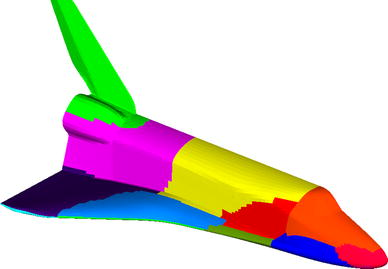
\includegraphics[width=0.95\linewidth]{fig3.jpg}
  \caption{Element-based domain decomposition of a surface mesh into 16 subdomains \cite{kirk2006}.}
  \vspace{-0.6em}
  \label{fig:decomp}
\end{figure}
\FloatBarrier

\section{Objectives}

The proposed work will solve set of equations (1-5) in 2-D geometry (r-z) for well-studied \gls{MSRE}, verify and validate results with reference \cite{briggs_molten-salt_1964}. Moreover, strong and weak scaling will be performed to find out appropriateness using Moltres for heavy computing full-core analysis.  

Additionally, finite-difference parallel solver will be developed to solve one-group neutron diffusion equation for the 2-D case for cross-verification Moltres' results. 

Finally, strong and weak scaling study will be done for both codes to compare scalability finite-element and finite-difference methods. The proposed work will contribute to the coupled neutronics / thermal-hydraulics simualations for \glspl{MSR} and will provide information for future development of multiphysics parallel solver for this type of reactors.

\section{Parallelization}

MOOSE framework uses LibMesh finite element library to solve set of physics equations. Different 
finite element formulations may be applied including Galerkin, Petrov-Galerkin, and discontinuous
 Galerkin methods \cite{kirk2006}. Parallelism is achieved using domain decomposition through mesh partitioning,
 in which each processor contains the global mesh but in general computes only on a particular subset. 
 Parallel implicit linear systems are supported via an interface with the PETSc library. 

A standard non-overlapping domain decomposition approach is used in LibMesh to achieve data distribution 
on parallel computers as shown in Fig.~\ref{fig:decomp}. The elements in each subdomain are assigned to an individual processor. The two primary metrics in judging the quality of a partition are the subdomain mesh size and the number of "edge cuts" in the resulting partition. For a mesh composed of a single type of element, each subdomain should contain an equal number of elements so that the resulting domain decomposition is load balanced across all available processors. Usually, for \gls{MSR} simulation
 adaptive mesh refinement and coarsening (AMR/C) scheme provided by LibMesh is employed. AMR/C allows do not explicitly specify domain decomposition, and provides optimal parallel performance with minimal user's efforts.
 
Developing C++/MPI code will employ finite-difference iterative method (i.e. Jacobi) to solve one-group neutron diffusion equation in 2-D mesh. Parallelization will be implemented using 2-D domain decomposition, when the 2D domain is divided
into multiple sub-domains using horizontal and/or vertical axis depending on the available number of computer nodes.

\begin{figure}[hbp!] % replace 't' with 'b' to 
  \centering
  \vspace{-0.3em}
  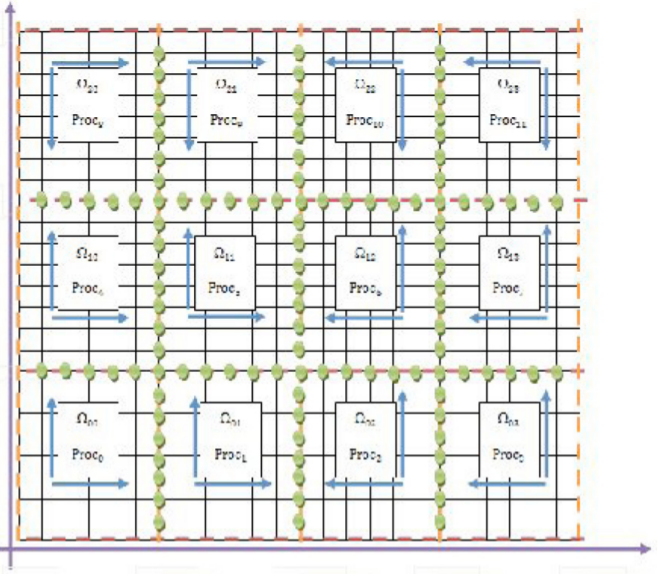
\includegraphics[width=0.85\linewidth]{domain_decomp.png}
  \caption{The division of $\Omega_n$ into 12 subdomains for 2-D case \cite{kirk2006}.}
  \vspace{-0.6em}
  \label{fig:domain_decomp}
\end{figure}
\FloatBarrier

For interior points neutron diffusion equation will be solved implicitly by Jacobi iterative scheme in combining with the boundary conditions. At the interface points of interior subdomains, equation will be solved by explicit iterative schemes. For illustration, consider a system N$_x$=N$_y$=24 with C=P$\times$Q = 3$\times$4 cluster nodes. The domain $\Omega_n$ can be decomposed to twelve subdomains as shown in Fig.~\ref{fig:domain_decomp}. The proposed approach fulfills the suitability for the implementation on Linux PC cluster through the minimization of inter-process communication by restricting the exchange of data to the interface between the sub-domains. To examine the efficiency and accuracy of the iterative algorithm, several numerical experiments using different number of nodes of the Linux PC cluster will be tested. The performance metrics should clearly show the benefit of using multicore system in terms of execution time reduction and speedup with respect to the sequential running in a single core.

%%%%%%%%%%%%%%%%%%%%%%%%%%%%%%%%%%%%%%%%%%%%%%%%%%%%%%%%%%%%%%%%%%%%%%%%%%%%%%%%
\bibliographystyle{ans}
\bibliography{bibliography}
\end{document}

